\documentclass[12pt,a4paper]{scrartcl}
\usepackage[utf8]{inputenc}
\usepackage[english,russian]{babel}
\usepackage{amssymb,amsfonts}
\usepackage{amsmath,cite,enumerate}
\usepackage{float,indentfirst}
\usepackage{graphicx}
\usepackage{geometry} % Меняем поля страницы
\geometry{left=2cm}% левое поле
\geometry{right=1.5cm}% правое поле
\geometry{top=1cm}% верхнее поле
\geometry{bottom=2cm}% нижнее поле
\graphicspath{{images/}}

\begin{document}


\begin{titlepage}
  \begin{center}
    Санкт-Петербургский Политехнический Университет     Петра Великого \\
    
    Институт компьютерных наук и технологий \\
    
    Кафедра компьютерных систем и программных технологий
  \end{center}
  
  \vfill
  
  \begin{center}
  Лабораторная работа №1\\
  по теме\\
  "Сигналы телекоммуникационных
систем"\\
\end{center}

\vfill

\newlength{\ML}
\settowidth{\ML}{«\underline{\hspace{0.7cm}}» \underline{\hspace{2cm}}}
\hfill\begin{minipage}{0.4\textwidth}
  Выполнил студент группы 33501/3\\
  \underline{\hspace{\ML}} Кисличенко Б.\,Д\\
\end{minipage}%

\bigskip

\settowidth{\ML}{«\underline{\hspace{0.7cm}}» \underline{\hspace{2cm}}}
\hfill\begin{minipage}{0.4\textwidth}
  Руководитель\\
  \underline{\hspace{\ML}} Богач Н.\,В\\
\end{minipage}%

\vfill
 
\begin{center}
  Санкт-Петербург\\
2018 
\end{center}

\end{titlepage}

\section{Цель}
\label{sec:goal}

Познакомиться со средствами генерации сигналов и визуализации их спектров.\\

\section{Постановка задачи}
\label{sec:task}

В командном окне MATLAB и в среде Simulink промоделировать синусоидальный и прямоугольный сигналы с различными параметрами. Получить их спектры. Вывести на график.\\

\section{Теоретический раздел}
\label{sec:teoriya}
Спектром сигнала обычно называют функцию, показывающую
зависимость интенсивности различиых гармоник в составе сигнала от частоты этих гармоник. Спектр периодического сигнала - это зависимость коэффициентов ряда Фурье от частот гармоник, которым эти коэффициенты соответствуют.\\
\\
Для непериодического сигнала спектр - это преобразование
Фурье сигнала. Итак. спектр периодического сигнала - это дискретный спектр (дискретная функция частоты), в то время как для непериодического сигнала характерен непрерывный спектр.

\section{Ход работы}
\label{sec:work}

\subsection{Работаем в Matlab}
\label{sec:workMatlab}

t=0:0.1:10;\\
A=1;\\
w=5;\\
fa=5;\\

y=A*sin(w*t+fa);\\

figure;\\
hold on;\\
axis([0 100 -inf inf])\\
axis square\\
grid on\\
plot(y);\\
hold off;\\

figure;\\
hold on;\\
axis square\\
grid on\\
plot(abs(fft(y,512)));\\
hold off;\\

Результат работы программы - на рис.1 и 2

\newpage
%Рисунок 1
\begin{figure}[h!]
\center{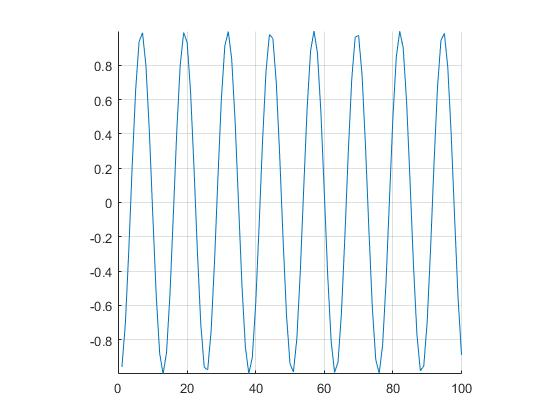
\includegraphics[width=0.6\linewidth]{sin155}}
\caption{Cинусоидальный сигнал с амлитудой 1, циклической частотой 5, начальной фазой 5.}
\end{figure}

%Рисунок 2
\begin{figure}[h!]
\center{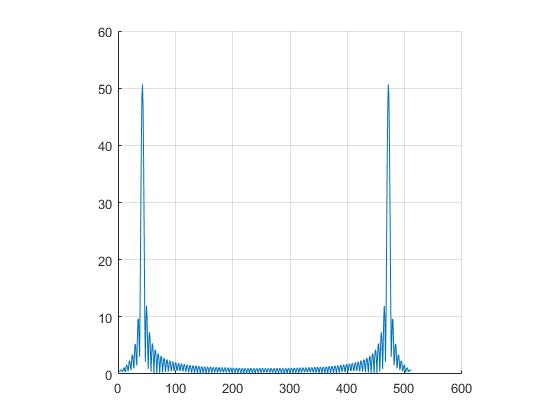
\includegraphics[width=0.6\linewidth]{sin155sp}}
\caption{Спектр синусоидального сигнала с амлитудой 1, циклической частотой 5, начальной фазой 5.}
\end{figure}

\textbf{Изменяем параметры:\\\\}
t=0:0.1:10;\\
A=2;\\
w=20;\\
fa=25;\\
y=A*sin(w*t+fa);\\
figure;\\
hold on;\\
axis([0 100 -inf inf])\\
axis square\\
grid on\\
plot(y);\\
hold off;\\
hold on;\\
axis square\\
grid on\\
plot(abs(fft(y,512)));\\
hold off;\\

%Рисунок 3
\begin{figure}[h!]
\center{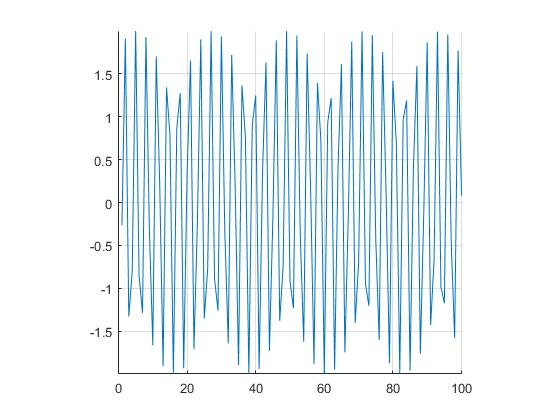
\includegraphics[width=0.6\linewidth]{sin2-20-25}}
\caption{Cинусоидальный сигнал с амлитудой 2, циклической частотой 20, начальной фазой 25.}
\end{figure}

%Рисунок 4
\begin{figure}[h!]
\center{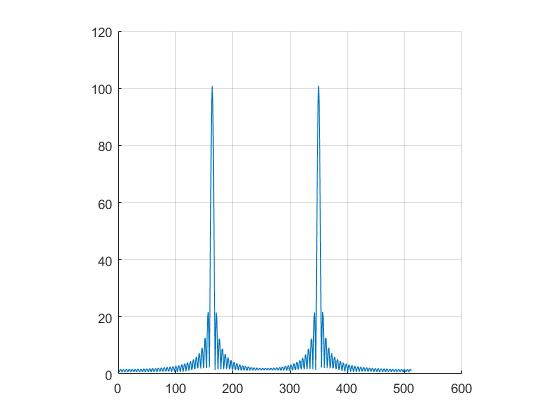
\includegraphics[width=0.6\linewidth]{sin2-20-25sp}}
\caption{Спектр синусоидального сигнала с амлитудой 2, циклической частотой 20, начальной фазой 25.}
\end{figure}

\newpage
\textbf{Создадим прямоугольный импульс:\\\\}
duty=20;\\
A=1;\\

y=A*square(2*t,duty);\\

figure;\\
hold on;\\
axis([0 100 -inf inf])\\
axis square\\
grid on\\
plot(y);\\
hold off;\\

figure;\\
hold on;\\
axis square\\
grid on\\
plot(abs(fft(y,512)));\\
hold off;\\

%Рисунок 5
\begin{figure}[h!]
\center{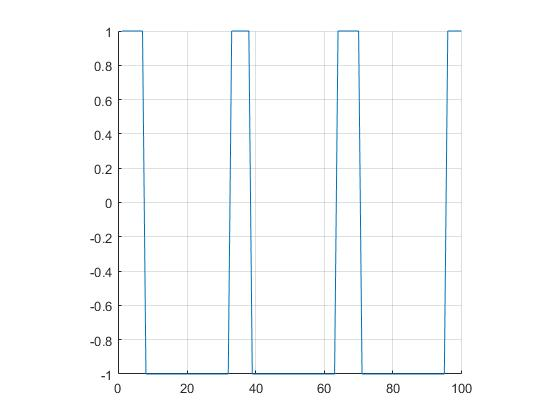
\includegraphics[width=0.6\linewidth]{square1-2-20}}
\caption{Прямоугольный сигнал с амлитудой 1, циклической частотой 2, duty=20.}
\end{figure}
\newpage

%Рисунок 6
\begin{figure}[h!]
\center{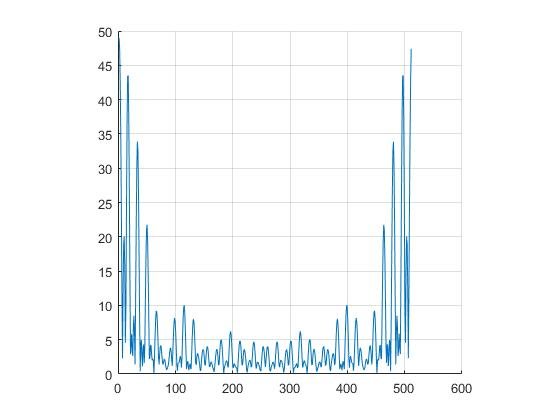
\includegraphics[width=0.6\linewidth]{square1-2-20sp}}
\caption{Спектр прямоугольного сигнала с амлитудой 1, циклической частотой 2, duty=20.}
\end{figure}

\textbf{Изменим параметры прямоугольного импульса:\\\\}
duty=40;\\
A=1.5;\\

y=A*square(1*t,duty);\\

figure;\\
hold on;\\
axis([0 100 -inf inf])\\
axis square\\
grid on\\
plot(y);\\
hold off;\\

figure;\\
hold on;\\
axis square\\
grid on\\
plot(abs(fft(y,512)));\\
hold off;\\

%Рисунок 7
\begin{figure}[h!]
\center{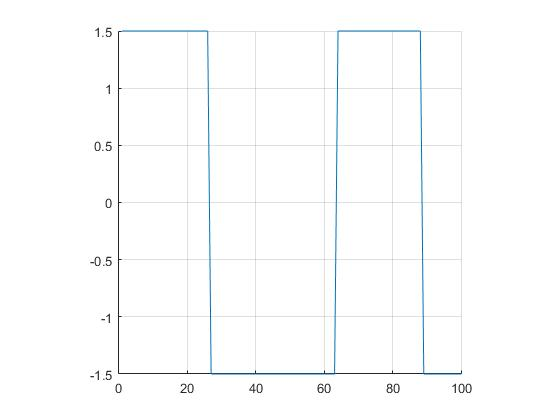
\includegraphics[width=0.6\linewidth]{square3d2-1-40}}
\caption{Прямоугольный сигнал с амлитудой 1.5, циклической частотой 1, duty=40}
\end{figure}

%Рисунок 8
\begin{figure}[h!]
\center{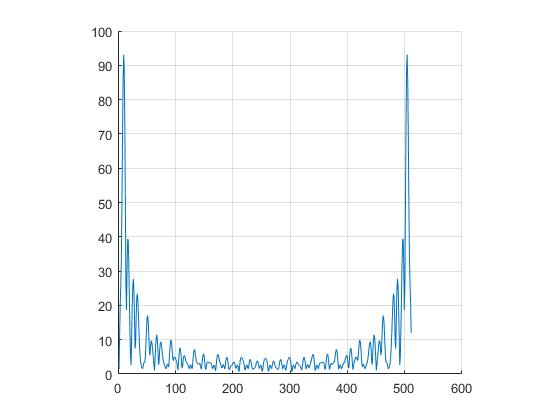
\includegraphics[width=0.6\linewidth]{square3d2-1-40sp}}
\caption{Спектр прямоугольного сигнала с амлитудой 1.5, циклической частотой 1, duty=40}
\end{figure}
\newpage

\subsection{Работаем в Simulink}
\label{sec:workSim}

%Рисунок 9
\begin{figure}[h!]
\center{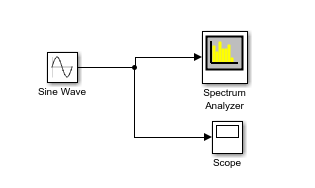
\includegraphics[width=0.4\linewidth]{simulink_sin}}
\caption{Cхема для синусоиды.}
\end{figure}

%Рисунок 10
\begin{figure}[h!]
\center{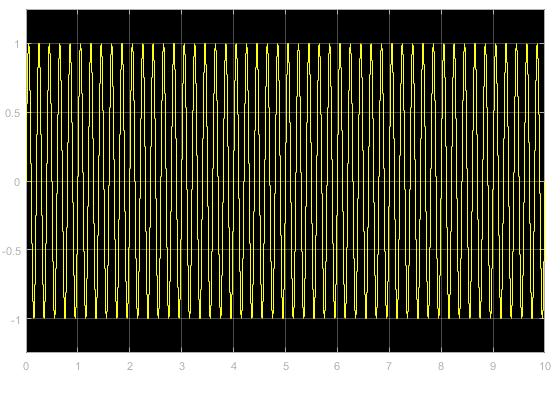
\includegraphics[width=\linewidth]{simulink1-0-200sin}}
\caption{Сигнал в Simulink.}
\end{figure}

\newpage
%Рисунок 11
\begin{figure}[h!]
\center{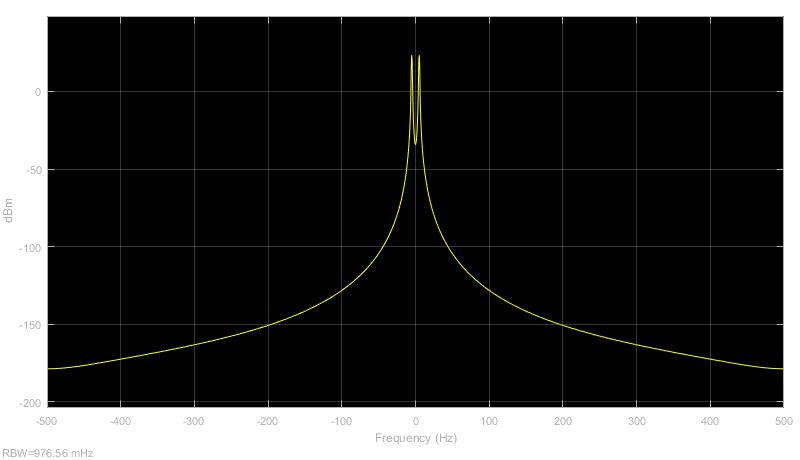
\includegraphics[width=\linewidth]{simulink1-0-200sin_sp}}
\caption{Спектр синусоиды в Simulink.}
\end{figure}

%Рисунок 12
\begin{figure}[h!]
\center{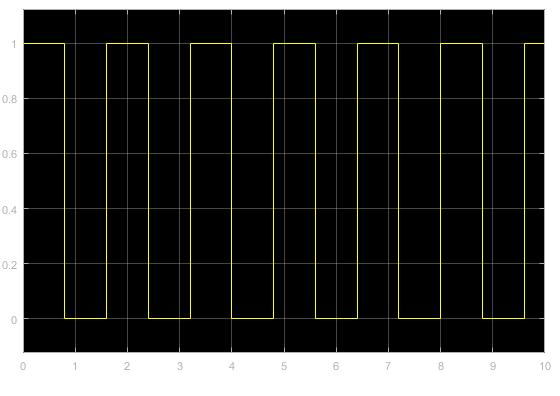
\includegraphics[width=\linewidth]{square1-1600-800-0-00d1simulink}}
\caption{Прямоугольный сигнал в Simulink.}
\end{figure}

%Рисунок 13
\begin{figure}[h!]
\center{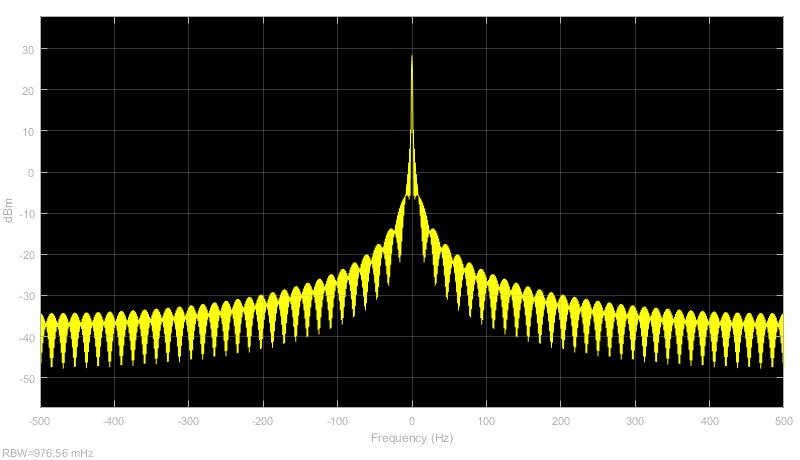
\includegraphics[width=\linewidth]{square1-1600-800-0-00d1simulink_sp}}
\caption{Спектр прямоугольного сигнала в Simulink.}
\end{figure}
\newpage

\section{Вывод}
\label{sec:afterWork}
В ходе данной лабораторной работы мы познакомились со средствами генерации и визуализации простых сигналов. Были построены синусоида и прямоугольный импульсный сигнал непосредственно в среде Matlab, а также в Simulink.\\
\\
Классификация сигналов осуществляется на основании существенных признаков соответствующих математических моделей сигналов. Все сигналы разделяют на две крупных группы: детерминированные и случайные. Детерминированные разделяются на переодические и непереодические(импульсые). К периодическим относят гармонические и полигармонические (сумма гармонических) сигналы. К непериодическим сигналам относят почти периодические и апериодические сигналы. Почти периодические сигналы близки по своей форме к полигармоническим. Они также представляют собой сумму двух и более гармонических сигналов (в пределе – до бесконечности), но не с кратными, а с произвольными частотами, отношения которых (хотя бы двух частот минимум) не относятся к рациональным числам. Апериодические сигналы составляют основную группу непериодических сигналов и задаются произвольными функциями времени.\\
\\
Случайные сигналы подразделяют на стационарные и нестационарные. Случайные стационарные сигналы сохраняют свои статистические характеристики в последовательных реализациях случайного процесса. Что касается случайных нестационарных сигналов, то их общепринятой классификации не существует.
\end{document}